\section{Qualitätssicherung}
\label{sec:Qualitätssicherung}

\subsection{PDCA-Zyklus}
\label{sec:PDCA-Zyklus}

Quelle: der-prozessmanager.de \cite{pdcaZyklus}

Der PDCA-Zyklus (auch Deming-Kreis, Deming-Zyklus oder PDCA Kreislauf) bezeichnet ein grundlegendes Konzept im kontinuierlichen Verbesserungsprozess. Es dient der Weiterentwicklung von Produkten und Dienstleistungen sowie bei der Fehler-Ursache-Analyse. Der PDCA-Kreis besteht aus den vier sich wiederholenden Phasen: \hl{Plan-Do-Check-Act} (dt. Planen – Umsetzen – Überprüfen – Handeln). 

\begin{center}
	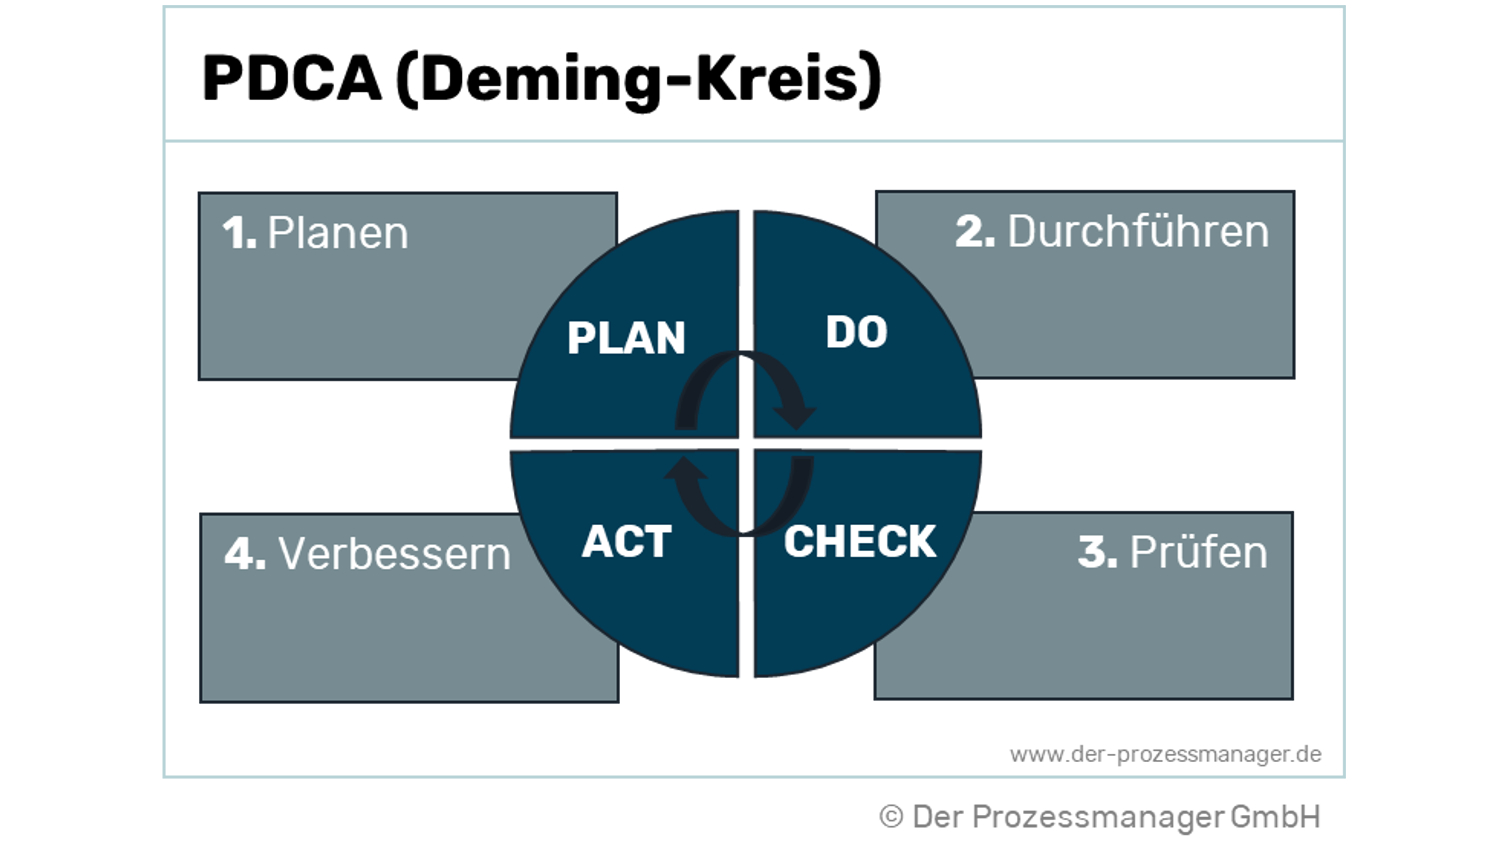
\includegraphics[scale=0.3]{Bilder/PDCA.png}
\end{center}

\textbf{Vorteile des PDCA-Kreises}

Der wesentliche Vorteil der PDCA-Methode ist wohl die \hl{einfache Anwendbarkeit}. Das Vorgehen hinsichtlich der spezifischen Aufgaben und Problemstellungen kann nahezu uneingeschränkt angepasst werden. Mit den Schritten Plan, Do, Check und Act bleibt dennoch ein solides Gerüst bestehen.

Weitere Vorteile:

\begin{itemize}
	\item Benötigt wenig Anleitung auf Grund des einfachen Aufbaus
	\item Die kreisförmige Konzeption ermöglicht ständige Verbesserung
	\item Durch den iterativen Ansatz lässt der PDCA-Zyklus Kontrolle und Analyse zu
\end{itemize}

\textbf{Nachteile des PDCA-Kreises}

Der große Vorteil des Demingkreises ist gleichzeitig auch ein wesentlicher Nachteil: \hl{Schnelle Problemlösungen lassen sich mit Hilfe des PDCA-Zyklus nicht umsetzen}.

Nachteile auf einen Blick:

\begin{itemize}
	\item Unklare Definition der einzelnen Schritte kann zu falschem Einsatz führen
	\item Verbesserungen im Unternehmen müssen langfristig gedacht sein
	\item Eher ein reaktiver Ansatz, statt proaktiv
\end{itemize}

\subsection{Incident Management}
\label{sec:IncidentManagement}

\todo{Fehlt}

Quelle: it-processmaps.com \cite{incidentManagement}

\subsection{Service Level Agreement (SLA), Servicelevel 1-3}
\label{sec:ServiceLevelAgreement}


\subsection{Testen}
\label{sec:Testen}

\subsubsection{Klassifizierung von Testverfahren}
\label{sec:KlassifizierungTestverfahren}

\begin{itemize}
	\item Wer testet?
	\begin{itemize}
		\item Mensch (manuell) vs. Maschine (automatisch)
		\item Entwickler vs. Benutzer
	\end{itemize}
	\item Was wird getestet?
	\begin{itemize}
		\item Komponente (Unit-Test/Funktionstest/Klassentest) vs. Integration vs. System (End-to-End)
		\item Testpyramide
	\end{itemize}
	\item Wie wird getestet?
	\begin{itemize}
		\item Bottom-Up vs. Top-Down
		\item statisch (Kompilierzeit) vs. dynamisch (Laufzeit)
		\item ohne Kenntnis des Codes (Blackbox) vs. mit Kenntnis des Codes (Whitebox)
		\item explorativ
		\item Schreibtischtest/Review
	\end{itemize}
	\item Wann wird getestet?
	\begin{itemize}
		\item Vor vs. nach der Entwicklung
		\item Abnahmetest
	\end{itemize}
	\item Warum wird getestet?
	\begin{itemize}
		\item Regressionstest
		\item Lasttest/Belastungstest
		\item Smoketest
	\end{itemize}
\end{itemize}



\subsection{Versionsverwaltung}
\label{sec:Versionsverwaltung} 


